\documentclass[10pt]{article}

\usepackage[margin=0.75in]{geometry}
\usepackage{amsmath,amsthm,amssymb,bm}
\usepackage{xcolor}
\usepackage{cancel}
\usepackage{graphicx}
\usepackage{changepage}
\usepackage{circuitikz}
\usepackage{pgfplots}
\usepackage{minted}
\usepackage{physics}
\usepackage{tikz}
\usepackage{tikz-3dplot}
\usepackage{hyperref}
\usepackage{cleveref}
\usepackage{siunitx}
\usepackage{fontspec}
\usepackage{relsize}
\usepackage{subfig}
\usepackage{todonotes}
\usepackage{contour}
\usepackage{multicol, multirow, booktabs}
\usepackage[breakable]{tcolorbox}
\usepackage[inline]{enumitem}

\theoremstyle{definition}
\newtheorem{problem}{Problem}
\newtheorem{soln}{Solution}

\pgfplotsset{compat=newest}
\usetikzlibrary{lindenmayersystems}
\usetikzlibrary{arrows}
\usetikzlibrary{calc}
\usetikzlibrary{positioning, fit}
\usetikzlibrary{3d, perspective}
\usetikzlibrary{math}
\usetikzlibrary{fadings}
\usetikzlibrary{angles,quotes} 
\usetikzlibrary{decorations.markings}

\definecolor{incolor}{HTML}{303F9F}
\definecolor{outcolor}{HTML}{D84315}
\definecolor{cellborder}{HTML}{CFCFCF}
\definecolor{cellbackground}{HTML}{F7F7F7}
\newcommand{\ui}{\hat{i}}
\newcommand{\uj}{\hat{j}}
\newcommand{\uk}{\hat{k}}
\newcommand{\ux}{\hat{\mathbf{x}}}
\newcommand{\uy}{\hat{\mathbf{y}}}
\newcommand{\uz}{\hat{\mathbf{z}}}
\newcommand{\uv}[1]{\hat{\bv{{#1}}}}
\newcommand{\pr}[1]{{#1^\prime}}
\newcommand{\pd}[2][]{{\frac{\partial^{#1}}{\partial {{#2}^{#1}}}}}
\newcommand{\dif}[2][]{{\frac{d^{#1}}{d{{#2}^{#1}}}}}
\newcommand{\grd}{\nabla}

\pgfdeclarelayer{background}  
\pgfsetlayers{background,main}
\AtBeginDocument{\RenewCommandCopy\qty\SI}

\makeatletter
\newcommand{\boxspacing}{\kern\kvtcb@left@rule\kern\kvtcb@boxsep}
\makeatother
\newcommand{\prompt}[4]{
    \ttfamily\llap{{\color{#2}[#3]:\hspace{3pt}#4}}\vspace{-\baselineskip}
}

\newcommand{\thevenin}[2]{
  \begin{center}
    \begin{circuitikz} \draw
      (0,0) -- (2,0) to[battery1, l_=$V_{Th}\eq#1$] (2,2) 
      to[resistor, l_=$R_{Th}\eq#2$] (0,2)
      ;
      \draw [o-] (-.07,2.079);
      \draw [o-] (-.07,0.079);
    \end{circuitikz}
  \end{center}
}

\newcommand{\norton}[2]{
  \begin{center}
    \begin{circuitikz} \draw
      (0,0) -- (3,0) to[american current source, l_=$I_{N}\eq#1$] (3,2) -- (0,2) (2,0)
      to[resistor, l=$R_{N}\eq#2$] (2,2)
      ;
      \draw [o-] (-.07,2.079);
      \draw [o-] (-.07,0.079);
    \end{circuitikz}
  \end{center}
}

\DeclareMathOperator{\Div}{div}
\DeclareMathOperator{\Curl}{curl}
\DeclareMathOperator{\sgn}{sgn}

\newcommand{\highlight}[1]{\colorbox{yellow}{$\displaystyle #1$}}
\newcommand{\ti}[1]{\widetilde{#1}}
\renewcommand{\div}[1]{\bv{\nabla}\cdot #1}
\renewcommand{\curl}[1]{\bv{\nabla}\times #1}

\newfontface{\Kaufmann}{Kaufmann}
\DeclareTextFontCommand{\kf}{\Kaufmann}
\newcommand{\scriptr}{\fontsize{12pt}{12pt}\kf{r}\fontsize{10pt}{10pt}}

\newfontface{\KaufmannB}{Kaufmann Bold}
\DeclareTextFontCommand{\kfb}{\KaufmannB}
\newcommand{\bscriptr}{\fontsize{12pt}{12pt}\kfb{r}\fontsize{10pt}{10pt}}
\newcommand{\justif}[2]{&{#1}&\text{#2}}
\newcommand{\bv}[1]{\bm{\mathrm{#1}}}

\title{Physics 4220H: Assignment II}
\author{Jeremy Favro (0805980) \\ Trent University, Peterborough, ON, Canada}
\date{\today}

\begin{document}
\maketitle

% PROBLEM 1
\begin{problem}
The intensity of sunlight hitting the earth is about $\qty{1300}{\watt\per\meter\squared}$. If sunlight strikes a
perfect absorber, what pressure does it exert? What about a perfect reflector?
Comment on the fraction of atmospheric pressure that the radiation pressure of
sunlight amounts to?
\end{problem}
\begin{soln}
  Coming straight from the formula in the text,
  $$P_{\text{radiation}}=\frac{1}{2}\epsilon_0E_0^2=\frac{I}{c}$$
  which for us is around $\qty{4.34e-6}{\pascal}$ for a perfect absorber, and since prefect reflectors
  get both the momentum from the initial impact and the turn-around momentum from reflection a perfect reflector would see a pressure of around
  $\qty{8.67e-6}{\pascal}$. Atmospheric pressure is roughly $\qty{10e5}{\pascal}$, $\num{1.18e10}$(!) times greater than the radiation pressure due to
  sunlight on a perfect reflector.
\end{soln}

% PROBLEM 2
\begin{problem}
You might be confused by the fact that the intensity of light in a linear medium,
$I=\epsilon_0cnE_0^2$, scales with the index of refraction and thus it is greater in the material
with the higher index. Consider Brewster's condition for TM light and compare the
intensities of the incident, reflected, and transmitted (refracted) waves. Comment
on the result.
\end{problem}
\begin{soln}
  At Brewster's angle all light is transmitted and since $T+R=1$, $T=1$ and so $I_I=I_T$, which is equivalent to saying that,
  for incident angle $\theta_B$ and transmitted angle $\theta_T$
  $$\frac{1}{2}\frac{n_1}{c\mu_1}E_{0I}^2\cos\theta_B=\frac{1}{2}\frac{n_2}{c\mu_2}E_{0T}^2\cos\theta_T.$$
  Cancelling common factors and taking the approximation that $\mu_1\approx\mu_2\approx \mu_0$,
  $$E_{0T}^2=\frac{n_1}{n_2}E_{0I}^2\frac{\cos\theta_B}{\cos\theta_T}.$$
  Since we are considering the case where $n_2>n_1$, the ratio $n_1/n_2<1$ and
  under the same condition Snell's law tells us that $\theta_T<\theta_B$ which equates to,
  for cosine between $0$ and $\pi/2$, $\cos\theta_T>\cos\theta_B$
  and hence the ratio $\cos\theta_B/\cos\theta_T<1$. These inequalities are preserved under a
  square root and so we can directly compare field amplitudes with
  $$E_{0T}=abE_{0I}$$
  where $a$ and $b$ are standins for the square roots of the ratios. My point is that both $a$ and $b$ are
  less than 1, and hence $E_{0T}<E_{0I}$, which is why the apparent issue with intensity is actually fine.
  The field scales down when entering an optically ``denser''(?) medium (one of the higher IOR)
  proportional to the angle at which it enters and the relative IORs, preserving overall intensity.
\end{soln}

% PROBLEM 3
\begin{problem}
Starting from the Fresnel equations for $E_{0R}/E_{0I}$ and $E_{0T}/E_{0I}$, show that energy is
conserved across the boundary, such that $T+R=1$. Do this both for TM and TE incidence.
\end{problem}
\begin{soln}
  \begin{enumerate}[label=(\alph*)]
    \item {\bf{TM}}: The Fresnel equations in this case tell us that
          $$E_{0R}=\frac{\alpha-\beta}{\alpha+\beta}E_{0I}\quad\text{ and }\quad E_{0T}=\frac{2}{\alpha+\beta}E_{0I}$$
          for $\alpha=\cos\theta_T/\cos\theta_I$ and $\beta\approx n_2/n_1$. Since intensity is, in general, given by
          $$I=\frac{1}{2}\epsilon v E_0^2$$
          the Fresnel equations give intensities
          $$I_I=\frac{1}{2}\epsilon_1 v_1 E_{0I}^2\cos\theta_I,
            \quad I_R=\frac{1}{2}\epsilon_1 v_1 \left(\frac{\alpha-\beta}{\alpha+\beta}\right)^2E_{0I}^2\cos\theta_I,
            \quad I_T=\frac{1}{2}\epsilon_2 v_2 \left(\frac{2}{\alpha+\beta}\right)^2E_{0I}^2\cos\theta_T
          $$
          where the cosines arise, as discussed in class, because we consider the amount of energy (or rather power) per unit
          area over the interface, not some plane at angle $\theta_I$ or $\theta_T$ to the interface-normal. Also note I've applied the law of reflected angles already.
          Now we consider (implicitly using the nonmagnetic approximation where appropriate)
          \begin{align*}
            I_R+I_T & =\frac{E_{0I}^2}{2}\left[\epsilon_1 v_1 \left(\frac{\alpha-\beta}{\alpha+\beta}\right)^2\cos\theta_I
            +\epsilon_2 v_2 \left(\frac{2}{\alpha+\beta}\right)^2\cos\theta_T\right]                                                             \\
                    & =\frac{E_{0I}^2}{2c\mu_0}\left[n_1\left(\frac{\alpha-\beta}{\alpha+\beta}\right)^2\cos\theta_I
            +n_2\left(\frac{2}{\alpha+\beta}\right)^2\cos\theta_T\right]                                                                         \\
                    & =\frac{E_{0I}^2}{2c\mu_0}\left[n_1\cos\theta_I\frac{\alpha^2-2\alpha\beta+\beta^2}{\alpha^2+2\alpha\beta+\beta^2}
            +\frac{4n_2\cos\theta_T}{\alpha^2+2\alpha\beta+\beta^2}\right]                                                                       \\
                    & =\frac{E_{0I}^2n_1\cos\theta_I}{2c\mu_0}\left[\frac{\left(n_1\cos\theta_I\right)\left(\alpha^2-2\alpha\beta+\beta^2\right)
                +4n_2\cos\theta_T
            }{\alpha^2+2\alpha\beta+\beta^2}\right]                                                                                              \\
                    & =\frac{E_{0I}^2n_1\cos\theta_I}{2c\mu_0}\left[\frac{\alpha^2-2\alpha\beta+\beta^2
                +4\alpha\beta
            }{\alpha^2+2\alpha\beta+\beta^2}\right]\justif{\quad}{Factor out $n_1\cos\theta_I$}                                                  \\
                    & =\frac{E_{0I}^2n_1\cos\theta_I}{2c\mu_0}\left[\cancelto{1}{\frac{\alpha^2+2\alpha\beta+\beta^2
            }{\alpha^2+2\alpha\beta+\beta^2}}\right]                                                                                             \\
                    & =\frac{1}{2}\frac{n_1}{2c\mu_0}E_{0I}^2\cos\theta_I
          \end{align*}
          and using $v=1/\sqrt{\epsilon\mu_0}$ and $v=c/n$,
          $$I_R+I_T=\frac{1}{2}\epsilon_1 v_1 E_{0I}^2\cos\theta_I=I_I.$$

    \item {\bf{TE}}: The Fresnel equations in this case tell us that
          $$E_{0R}=\frac{1-\alpha\beta}{1+\alpha\beta}E_{0I}\quad\text{ and }\quad E_{0T}=\frac{2}{1+\alpha\beta}E_{0I}$$
          for $\alpha=\cos\theta_T/\cos\theta_I$ and $\beta\approx n_2/n_1$. This gives us intensities
          $$I_I=\frac{1}{2}\epsilon_1 v_1 E_{0I}^2\cos\theta_I,
            \quad I_R=\frac{1}{2}\epsilon_1 v_1 \left(\frac{1-\alpha\beta}{1+\alpha\beta}\right)^2E_{0I}^2\cos\theta_I,
            \quad I_T=\frac{1}{2}\epsilon_2 v_2 \left(\frac{2}{1+\alpha\beta}\right)^2E_{0I}^2\cos\theta_T.
          $$
          Again we consider the sum of the reflected and transmitted intensities, using the nonmagnetic approximation where appropriate
          \begin{align*}
            I_R+I_T & =\frac{E_{0I}^2}{2c\mu_0}\left[
              n_1\left(\frac{1-\alpha\beta}{1+\alpha\beta}\right)^2\cos\theta_I
              +n_2 \left(\frac{2}{1+\alpha\beta}\right)^2\cos\theta_T
            \right]                                                  \\
                    & =\frac{E_{0I}^2}{2c\mu_0}\left[
              n_1\cos\theta_I\frac{1-2\alpha\beta+(\alpha\beta)^2}{1+2\alpha\beta+(\alpha\beta)^2}
              +n_2\cos\theta_T \frac{4}{1+2\alpha\beta+(\alpha\beta)^2}
            \right]                                                  \\
                    & =\frac{E_{0I}^2}{2c\mu_0}\left[
              \frac{\left(n_1\cos\theta_I\right)\left(1-2\alpha\beta+(\alpha\beta)^2\right)+4n_2\cos\theta_T}{1+2\alpha\beta+(\alpha\beta)^2}
            \right]                                                  \\
                    & =\frac{E_{0I}^2n_1\cos\theta_I}{2c\mu_0}\left[
              \frac{1-2\alpha\beta+(\alpha\beta)^2+4\alpha\beta}{1+2\alpha\beta+(\alpha\beta)^2}
            \right]                                                  \\
                    & =\frac{E_{0I}^2n_1\cos\theta_I}{2c\mu_0}\left[
              \cancelto{1}{\frac{1+2\alpha\beta+(\alpha\beta)^2}{1+2\alpha\beta+(\alpha\beta)^2}}
              \right]
          \end{align*}
          which, reworking as before, yields
          $$I_R+I_T=\frac{1}{2}\epsilon_1 v_1 E_{0I}^2\cos\theta_I=I_I.$$
  \end{enumerate}
\end{soln}

% PROBLEM 4
\begin{problem}
Boundary conditions yielded the following ``four'' equations for the case of TM
incidence:
\begin{align}
   & \epsilon_1(-E_{0I}+E_{0R})\sin\theta_I=-\epsilon_2E_{0T}\sin\theta_T \\
   & 0=0\, (\text{No $B_z$})                                              \\
   & (E_{0I}+E_{0R})\cos\theta_I=E_{0T}\cos\theta_T                       \\
   & \frac{1}{\mu_1v_1}(E_{0I}-E_{0R})=\frac{1}{\mu_2v_2}E_{0T}.
\end{align}
Draw a detailed diagram and derive the 4 equivalent equations for {\bf{TE}} incidence.
\end{problem}
\begin{soln}~
  \begin{center}
    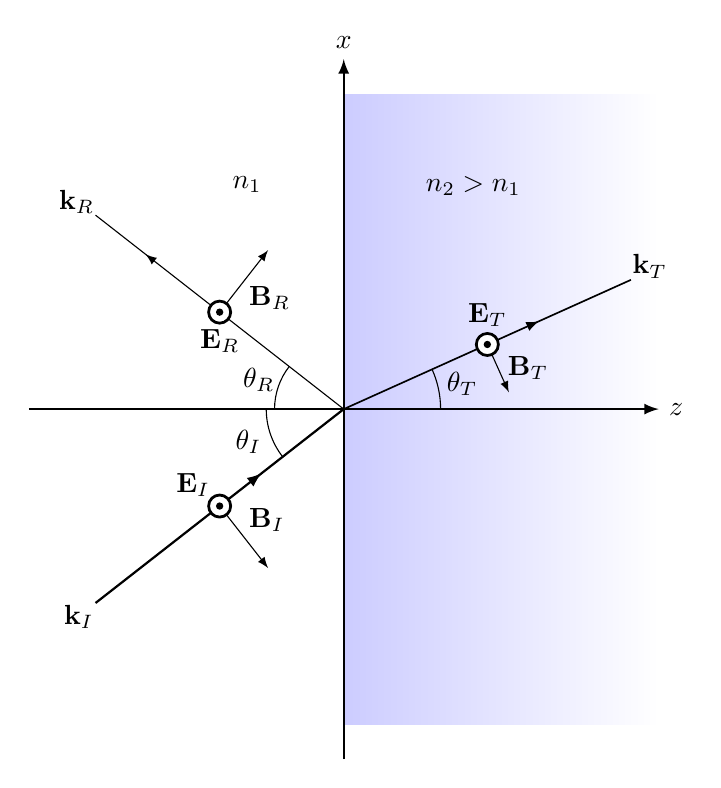
\begin{tikzpicture}[scale=2]
      \tikzset{
        pics/.cd,
        vector in/.style args={#1/#2}{
            code={
                \draw[#1] (0,0)  circle (1);
                \draw[#2] (45:1) -- (225:1) (135:1) -- (315:1);
              }
          }
      }
      \tikzset{
        pics/vector out/.style args={#1/#2}{
            code={
                \draw[line width=#1, fill=white] (0,0) circle (#2);
                \fill[black] (0,0) circle ({#2/3});
              }
          }
      }

      \def\H{4} % Interface height
      \def\t{2} % Interface thickness
      \def\l{2} % Ray length
      \def\IORI{1}
      \def\IORT{1.5}
      \def\thetaI{38}
      \def\thetaR{180-\thetaI}
      \def\thetaT{asin(\IORI*sin(\thetaI)/\IORT)}
      \coordinate (O) at (0, 0);
      \coordinate (I) at (180+\thetaI:\l);
      \coordinate (R) at (\thetaR:\l);
      \coordinate (T) at ({\thetaT}:\l);
      \coordinate (B) at (-\t, 0);
      \coordinate (Bp) at (\t, 0);

      \tikzset{
        light beam/.style={thick, black, decoration={markings,
                mark=at position #1 with {\arrow{latex}}},
            postaction={decorate}},
        light beam/.default=0.5}

      \shade[top color=blue!20,bottom color=white,shading angle=90] (0,\H/2) rectangle++ (\t,-\H); % glass
      \node[below left=1.3] at (0,\H/2) {$n_1$};
      \node[below right=1.3] at (0,\H/2) {$n_2>n_1$};
      \draw[-latex, thick] (-\t,0) -- (\t,0) node[right]{$z$};
      \draw[-latex, thick] (0,-\H/1.8) -- (0,\H/1.8) node[above]{$x$};

      % Rays
      \draw[light beam={0.67}] (I) node[below left=-0.15]{$\bv{k}_I$} -- (O); % incoming ray
      \draw[-latex] ($(I)!0.5!(O)$) -- +({atan(-1/tan(\thetaI))}:{\l/4}) node[midway, above right=-0.08] {$\bv{B}_I$};
      \path ($(I)!0.5!(O)$) pic {vector out=1pt/.14} node[above left] {$\bv{E}_I$};

      \draw[light beam={0.8},line width=0.4] (O) -- (R) node[above left=-0.15]{$\bv{k}_R$}; % reflected ray
      \draw[-latex] ($(O)!0.5!(R)$) -- +({atan(-1/tan(\thetaR))}:{\l/4}) node[midway, below right=-0.08] {$\bv{B}_R$};
      \path ($(O)!0.5!(R)$) pic {vector out=1pt/.14} node[below=0.1] {$\bv{E}_R$};

      \draw[light beam={0.68},line width=0.6] (O) -- (T) node[above right=-0.15]{$\bv{k}_T$}; % refracted ray
      \draw[-latex] ($(O)!0.5!(T)$) -- +({atan(-1/tan(\thetaT))}:{\l/6}) node[midway, right] {$\bv{B}_T$};
      \path ($(O)!0.5!(T)$) pic {vector out=1pt/.14} node[above=0.1] {$\bv{E}_T$};

      % Angles
      \draw pic["$\theta_I$", draw=black, angle radius=28, angle eccentricity=1.3] {angle = B--O--I};
      \draw pic["$\theta_R$",draw=black,angle radius=25,angle eccentricity=1.3] {angle = R--O--B};
      \draw pic["$\theta_T$",draw=black,angle radius=35,angle eccentricity=1.25] {angle = Bp--O--T};
    \end{tikzpicture}
  \end{center}
  I am extremely proud of that diagram, now to actually solve the problem. I'll skip the first couple steps to obtain the laws of reflection and refraction
  and instead focus on applying boundary conditions,
  \begin{align}
    \epsilon_1(E_{0I}^\perp+E_{0R}^\perp)                               & =\epsilon_2E_{0T}^\perp \\
    \bv{E}_1^\parallel-\bv{E}_2^\parallel                               & =\bv{0}                 \\
    \frac{1}{\mu_1}\bv{B}_1^\parallel-\frac{1}{\mu_2}\bv{B}_2^\parallel & =\bv{K}_f\times\uv{n}   \\
    B_1^\perp-B_2^\perp                                                 & =0
  \end{align}
\end{soln}

% PROBLEM 5
\begin{problem}
In lecture, we analyzed the expressions we obtained for Fresnel coefficients $t$, $r$, $T$,
and $R$ to draw detailed plots of these parameters in the case of external reflection
(going from optically rare to optically dense media; $n_1<n_2$). Do the same thing for
the case of internal reflection (specifically for the case $n_1=1.5$, $n_2=1.3$; incidence
from glass into water), by attending to the following questions:
\begin{enumerate}[label=(\alph*)]
  \item Is there a critical angle for TIR (If so, what is it)?
  \item Is there a Brewster's angle for which there is no reflection (If so, what is it)?
  \item Is it possible for either/both $t$ and $r$ to exceed 1?
  \item At what value are $T$ and $R$ equal?
  \item Put all these ideas together and plot/sketch two detailed graphs (one for TE and one
        for TM) for $t$, $r$, $T$, and $R$ for internal reflection from glass into water.
  \item {[Bonus]} What can you say about the phase of the fields upon reflection in this
        case? Are there any $\pi$ flips? If so, at what angle(s)?
\end{enumerate}
\end{problem}
\begin{soln}

\end{soln}
\end{document}